\chapter{Experimental Infrastructure}

In this section, the hardware and frameworks used for this thesis will be described. The hardware used was mainly the ATLASCAR 2 and its sensors: two SICK LMS151 LIDAR, one SICK LD-MRS LIDAR and a PointGrey Zebra 2 Camera. The central framework that receives messages from the sensors is ROS (Robotic Operative System). This data will be processed using OpenCV for images, and several libraries will be used for the range-based sensors, such as PCL (Point Cloud Library) and MTT 

\section{ATLASCAR 2}

The ATLASCAR 2 is based in the platform of the 2015 Mitsubishi i-MiEV, a full electric vehicle. The battery that powers the engine is the same powering the camera and the sensors. The main characteristics of the car are in table \ref{tab: MiEV technical} \cite{MITSUBISHIMOTORS}. 

\begin{figure}[htp]
	
	\centering
	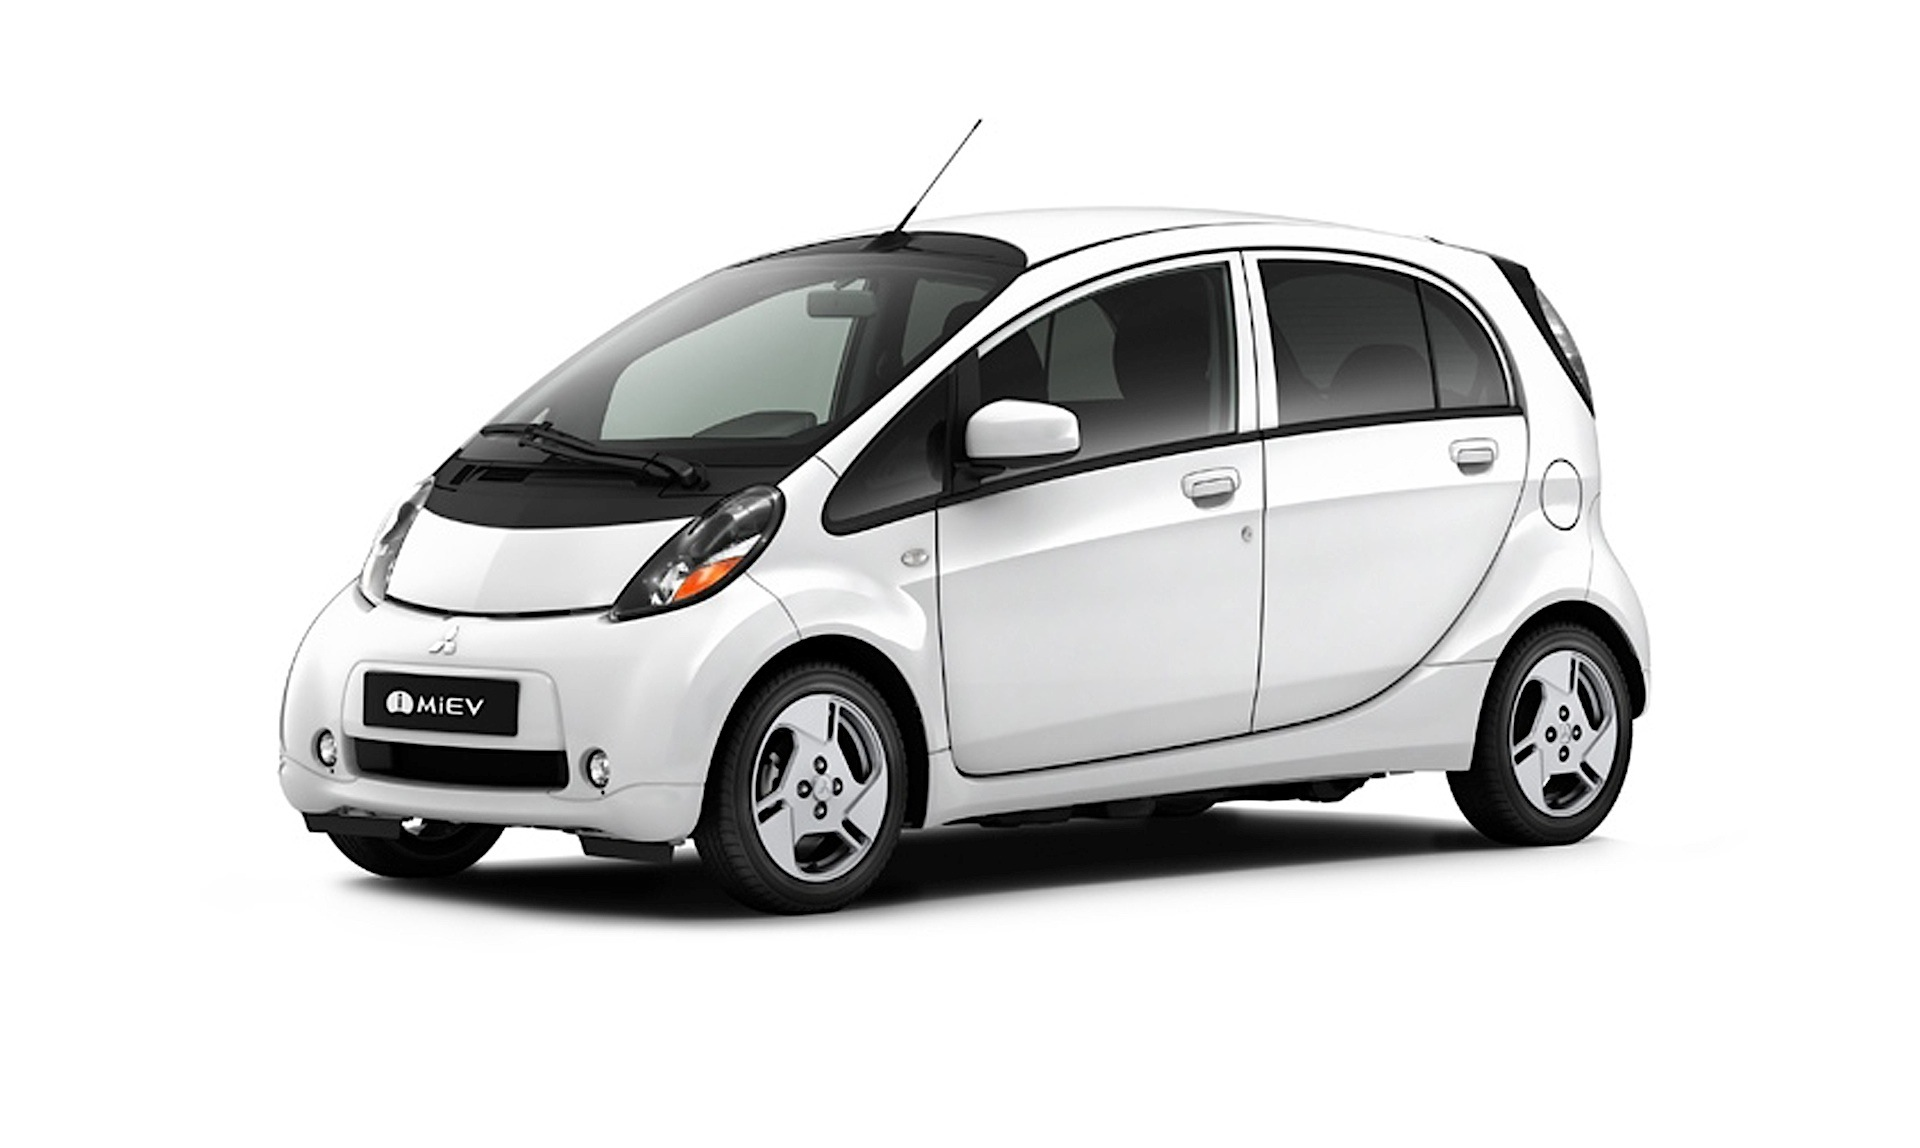
\includegraphics[width=.9\textwidth]{capexp/imgs/imiev}\hfill
	
	\caption{The Mitsubishi i-MiEV}
	\label{fig:imiev}
	
\end{figure}

\begin{table}[!h]
	\centering
	\caption{Mitsubishi i-MiEV technical specifications}
	\label{tab: MiEV technical}
	\begin{tabular}{lcc}
		Characteristic & Unit & Value\\
		Wheelbase & mm & 2550\\
		Track (Front/Rear) & mm & 1310/1270 \\
		Vehicle weight & kg  & 1450 \\
		\hline
		Engine & -- & Electric \\
		Electric energy consumption & Wh/km & 135 \\
		Electric range (NEDC)  & km & 150 \\
		Maximum speed & km/h & 130 \\
		Minimum turning radius & m & 4.5 \\
		Max. Power output & kW & 49 \\
		Max. torque & Nm & 180 \\
		\hline
		Traction battery type & -- & Lithium-ion battery \\
		Traction battery voltage & V & 330 \\
		Traction battery energy & kWh & 16 \\
		Regular charging (AC 230V 1 phase) 8A & hrs & 10 \\
	\end{tabular}
\end{table}

\section{Sensors}

The sensors equipped in the ATLASCAR 2 are two SICK LMS151 LIDAR, a SICK LD-MRS LIDAR and a PointGrey Zebra 2 Camera. It is of most importance for the ATLASCAR 2 to have this sensors to be capable of perception. The sensors have been mounted in the front of the car in an aluminum infrastructure designed by Correia. \cite{Correia2017}

\subsection{SICK LMS151 LIDAR}

The SICK LMS151 (figure \ref{fig:sicklms}) is a LIDAR sensor designed to be used in outdoors. It is a planar infrared scanner with a large planar aperture angle often used in robotics and in AD fields for its high scanning frequency and operating range. This scanner is also able to scan distances through fog, glass and dust (multi-echo technology). This scanner is provided with an Ethernet TCP/IP interface with high data transmission rate. \cite{SICK}

\begin{figure}[htp]
	
	\centering
	\hfill
	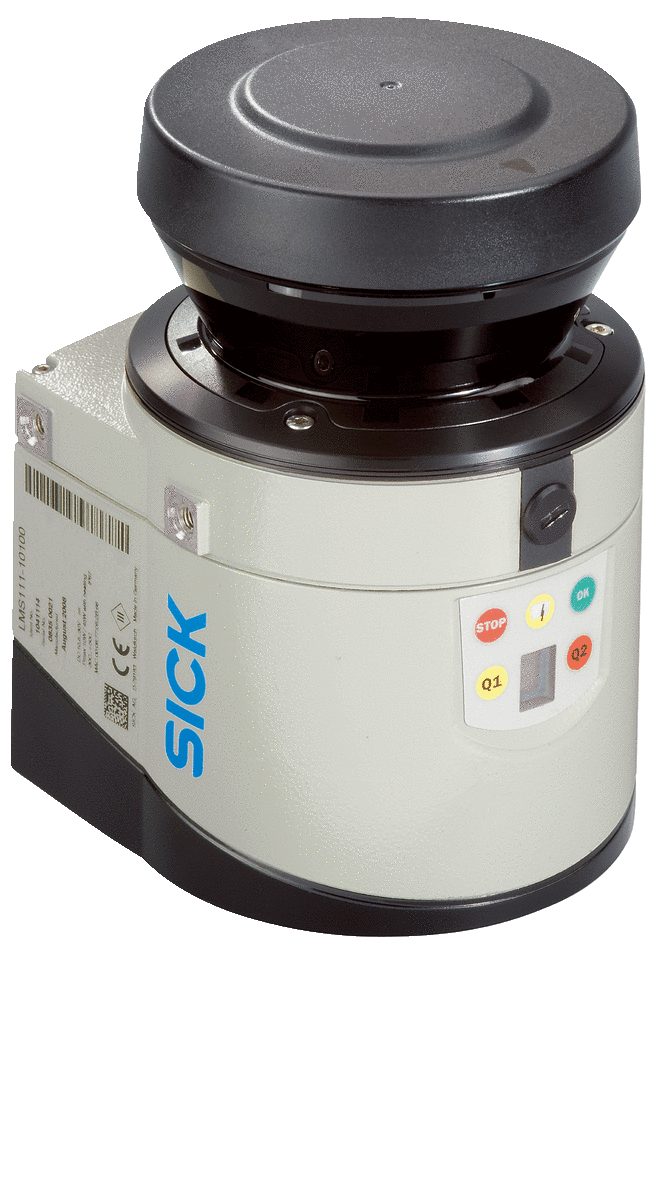
\includegraphics[width=.3\textwidth]{capexp/imgs/sicklms}\hfill
	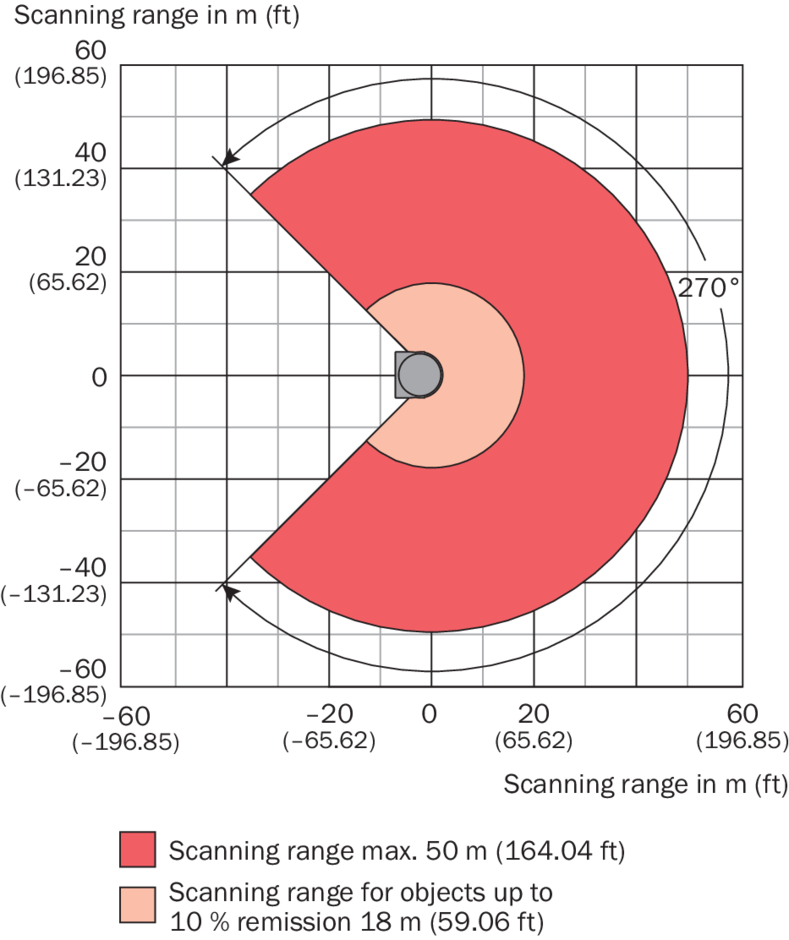
\includegraphics[width=.5\textwidth]{capexp/imgs/sicklms2}\hfill
	
	\caption{The SICK LMS151 LIDAR and its operating range}
	\label{fig:sicklms}
	
\end{figure}

\begin{table}[!h]
	\centering
	\caption{SICK LMS151 specifications}
	\label{tab: sicklmsspecs}
	\begin{tabular}{ll}
		\hline
		Field of application & Outdoors\\
		Laser Class & 	1 (IEC 60825-1:2014, EN 60825-1:2014) \\
		Aperture Angle & 270$^{\circ}$ \\
		Scanning frequency & 25 Hz / 50 Hz \\
		Angular resolution	& 0.25$^{\circ}$ / 0.5$^{\circ}$ \\
		Operating range	& 0.5 m ... 50 m \\
		Max. range with 10 \% reflectivity & 18 m \\
		Amount of evaluated echoes & 2 \\
		Data transmission rate & 10/100 MBit/s \\
		\hline
	\end{tabular}
\end{table}

For this project, the SICK LMS151 will operate at 50 Hz with an angle increment of 0.5$^{\circ}$ between readings. Each message will transmit a total of 540 points per scan in polar coordinates $(r,\theta)$. \cite{SICK}

\subsection{SICK LD-MRS LIDAR}

The SICK LD-MRS (figure \ref{fig:sickldmrs}) is a LIDAR sensor also designed to be used in outdoors. It features 4 planar infrared scanners with 0.8$^{\circ}$ vertical aperture angle between each plan, offering tri-dimensional point clouds. It provides high scanning frequencies and long operating range up to 300 meters. This scanner is also provided with an Ethernet TCP/IP interface with high data transmission rate. \cite{SICKa}

\begin{figure}[htp]
	
	\centering
	\hfill
	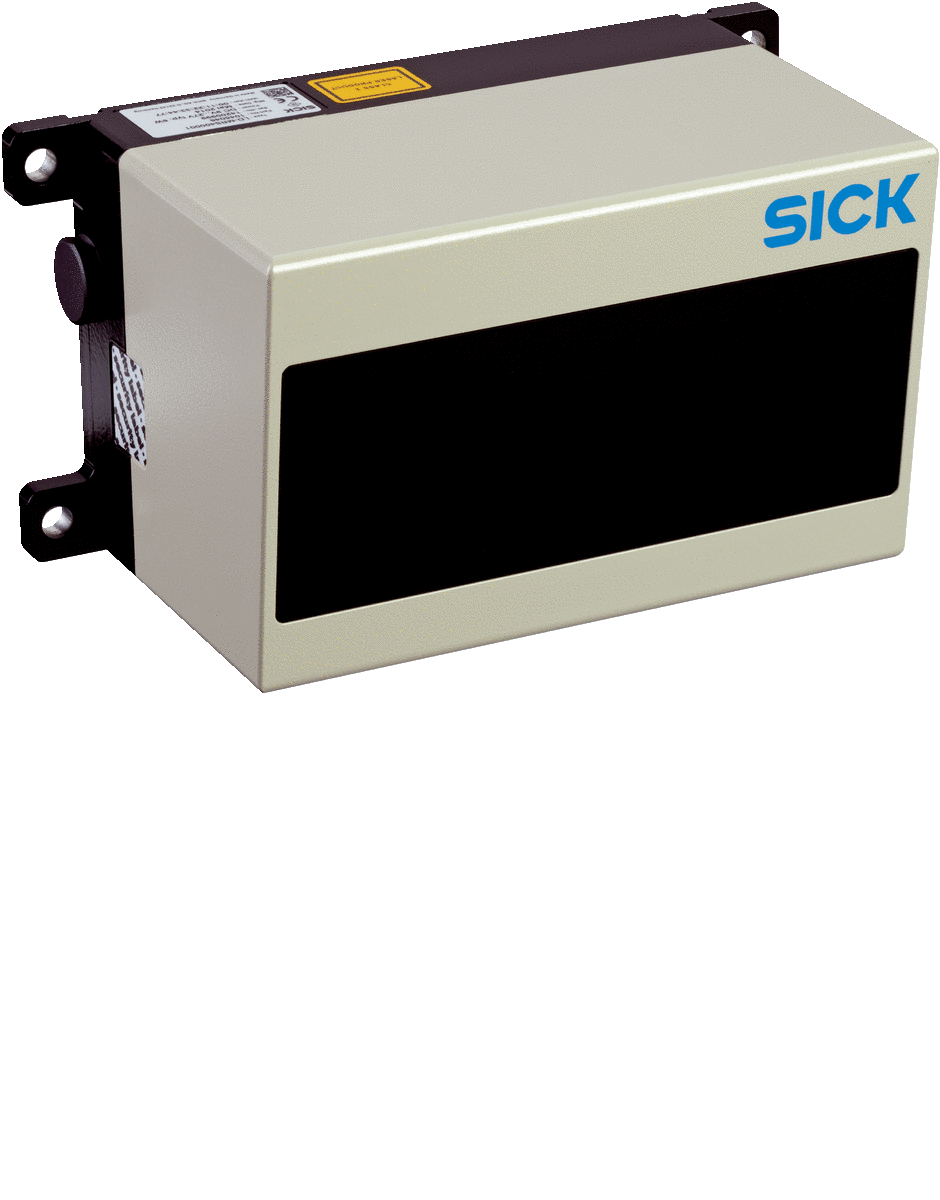
\includegraphics[width=.4\textwidth]{capexp/imgs/sickldmrs}\hfill
	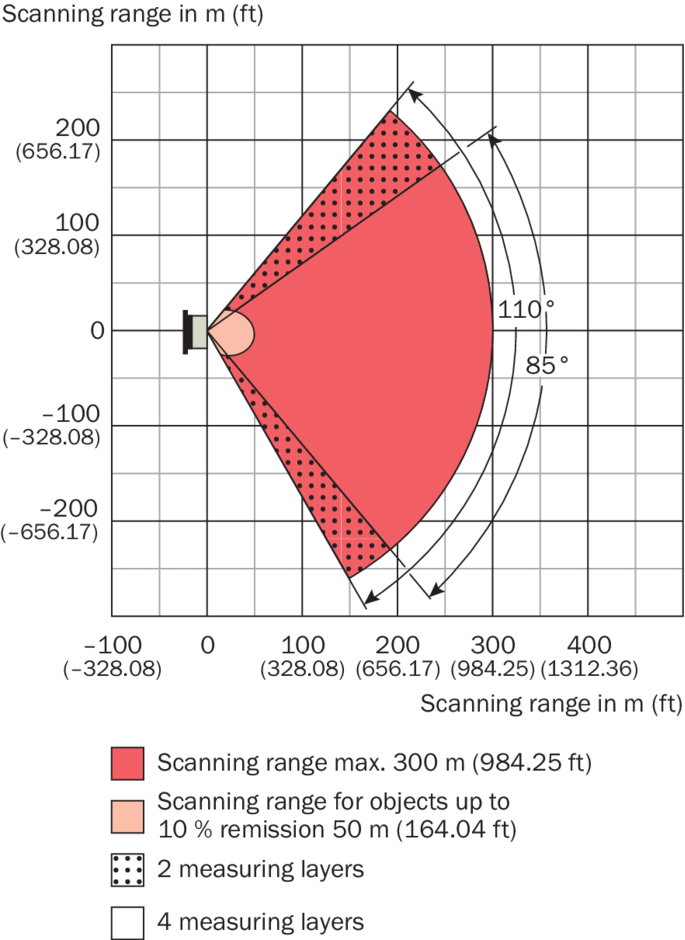
\includegraphics[width=.5\textwidth]{capexp/imgs/sickldmrs2}\hfill
	
	\caption{The SICK LD-MRS LIDAR and its operating range}
	\label{fig:sickldmrs}
	
\end{figure}

\begin{table}[!h]
	\centering
	\caption{SICK LMS151 specifications}
	\label{tab: sickldmrsspecs}
	\begin{tabular}{ll}
		\hline
		Field of application & Outdoors\\
		Laser Class & 	1 (IEC 60825-1:2014, EN 60825-1:2014) \\
		Scanner Planes & 4 measuring planes \\
		Aperture Angle & 85$^{\circ}$  \\
		Total Aperture & 110$^{\circ}$\\
		Scanning frequency & 12.5 Hz / 50 Hz \\
		Angular resolution	& 0.125$^{\circ}$ / 0.25$^{\circ}$ / 0.5$^{\circ}$ \\
		Operating range	& 0.5 m ... 300 m \\
		Max. range with 10 \% reflectivity & 50 m \\
		Amount of evaluated echoes & 3 \\
		Data transmission rate & 100 MBit/s \\
		\hline
	\end{tabular}
\end{table}

For this project, the SICK LD-MRS will operate at 50 Hz with an angle increment of 0.5$^{\circ}$ between readings. Each message will transmit a total of 200 points per scan in polar coordinates $(r,\theta)$ for each plan. Since this scanner offers four planar scans, the final point cloud will total 800 points. \cite{SICKa}

\subsection{PointGrey Zebra 2 Camera}

The PointGrey Zebra 2 Camera (figure \ref{fig:pointgrey}) is a high resolution camera with a Sony ICX274. It also features a GigE PoE Interface and it is highly configurable to fulfill any particular utilization needs. \cite{PointGrey} The camera is inserted in a case made with 3D printing and designed by Correira \cite{Correia2017}.  Other relevant specifications are found in table \ref{tab: pointgreyspecs}. 

\begin{figure}[htp]
	
	\centering
	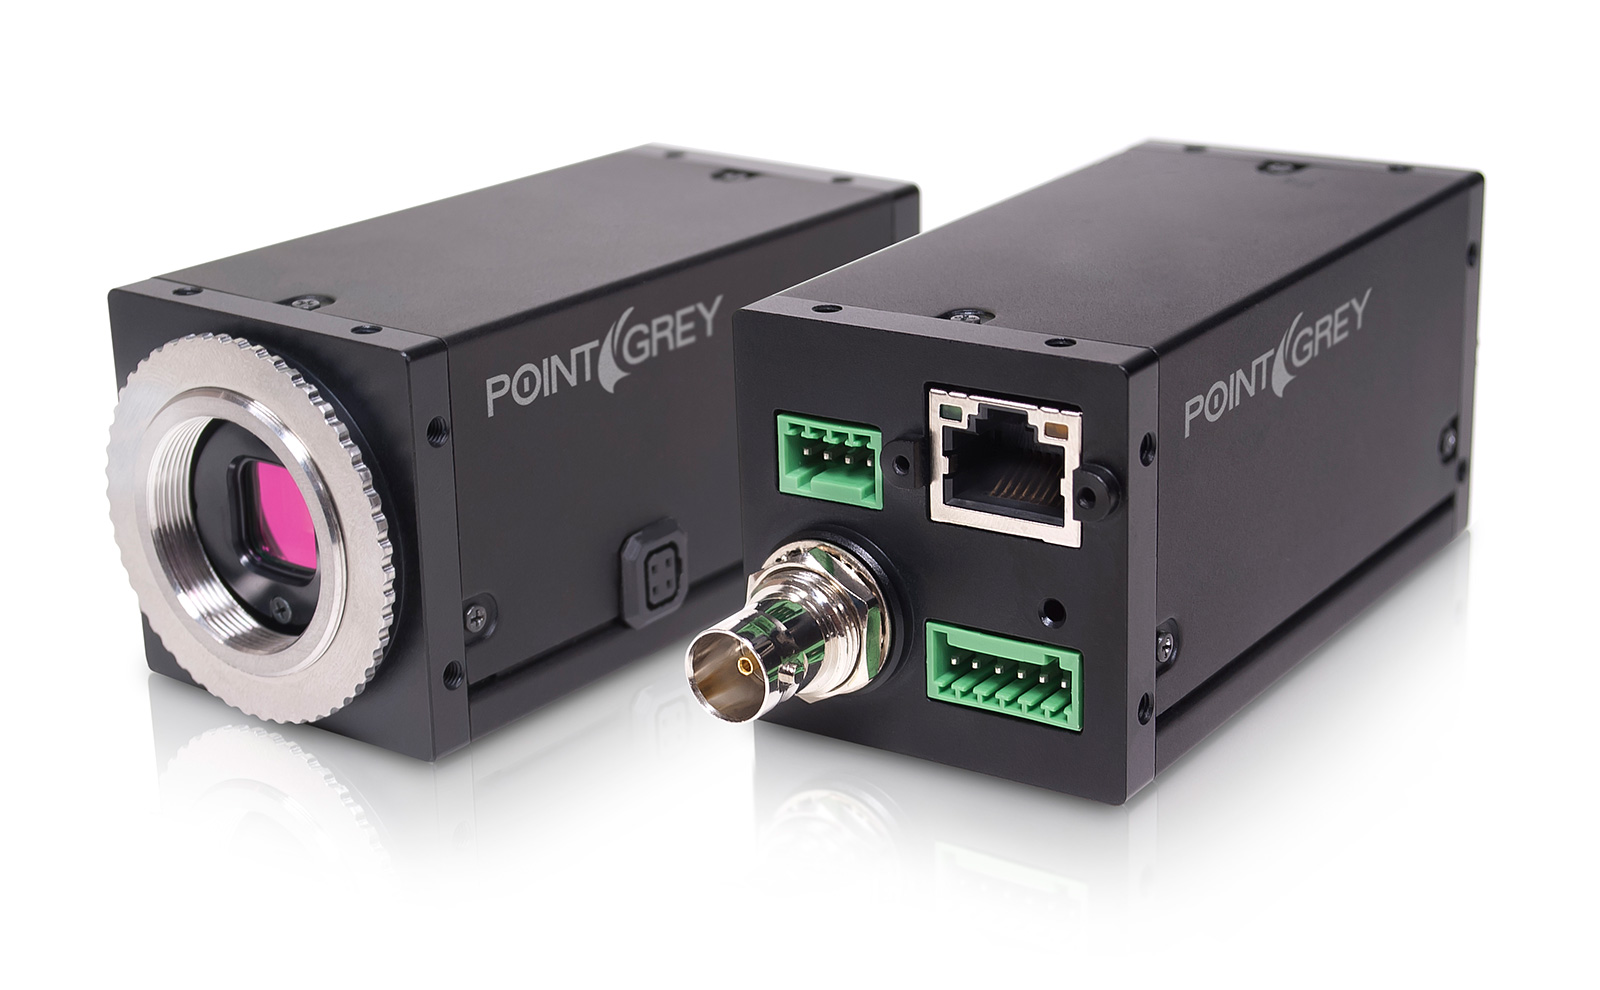
\includegraphics[width=.6\textwidth]{capexp/imgs/pointgrey}
	
	\caption{The PointGrey Zebra 2 Camera}
	\label{fig:pointgrey}
	
\end{figure}

\begin{table}[!h]
	\centering
	\caption{PointGrey Zebra 2 Camera specifications}
	\label{tab: pointgreyspecs}
	\begin{tabular}{ll}
		
		\hline
		Resolution & 1624 x 1224\\
		Max. Frame Rate & 25 FPS with HD-SDI \\
		Megapixels & 2.0 MP \\
		Chroma & Color\\
		Sensor & Sony ICX274 CCD \\
		Image Buffer &	32 MB\\
		Interface &	GigE PoE, HD-SDI\\
		
		\hline
	\end{tabular}
\end{table}

Working at maximum resolution and frame rate would saturate the network bandwidth and increase image processing times. In this project the camera's frame rate is set at 7.5 FPS so that a balance between image quality and processing optimization can be accomplished.


\section{Software}

In this section it will be discussed the software used in this dissertation. The base architecture of this dissertation is centered in the ROS framework. Many ROS tools and features are used such as Rviz, rosbags, roslaunch and rosrun. Two main nodes are to be developed in this work: the camera calibration package node (previously developed by Silva \cite{VieiradaSilva2016}) and the labelling node. The handling of data from the sensors was done using PCL, MTT, 
and the image processing was performed with OpenCV libs. All software was programmed with C++.

\section{ROS}
The central framework in the ATLASCAR 2 is based on ROS Kinect on Ubuntu 16.04. %Falar aqui um pouco sobre o ROS% 
With ROS it is possible to receive data packets and transform them in messages that contain data from the sensors. It is possible to manipulate this data using ROS nodes.

\subsection{Rviz}
Rviz is the standard ROS tool for visualization. %falar mais um pouco sobre o rviz%

The Rviz will be used to visualize data from the ATLASCAR 2 either directly in real-time or in rosbags. It will also serve as a debugging tool in which pointcloud values can be easily seen.

\subsection{Rosbag}
Rosbags are files in ROS used to simulate the workspace environment. In other words, it is possible to test the developed nodes without actually being in the ATLASCAR 2. %falar mais um pouco sobre os rosbags%5

\subsection{Roslaunch}
The roslaunch files are used to launch several nodes in ROS simultaneously. A roslaunch sets up a roscore (or ROS master), set parameters for the nodes, and can also execute other launch files. %falar mais um pouco dos roslaunch%

\subsection{Multi-sensor calibration package}

The multi-sensor calibration package is a package developed by Silva. The package contains a GUI used to calibrate the several sensors in the ATLASCAR 2. 